% !TeX root = ../document.tex
\documentclass[../document.tex]{subfiles}
\lstset{inputpath=sections}
\begin{document}

	\subsection{Maximal margin classifier}

	\paragraph{What is a hyperplane?}
	A hyperplane is a flat surface of dimension p-1 in a p dimensional space.
	\begin{equation}
		\beta_{0}+\beta_{1}X_{1}+\beta_{2}X_{2}+...+\beta_{p}X_{p}=0
	\end{equation}
	This plane cuts the p-space in half.

	\paragraph{Classification using a separating hyperplane}
	When the training data fall into two classes we can use a hyperplane to separate the data.
	\begin{equation}
		y_{i}(\beta_{0}+\beta_{1}x_{i1}+\beta_{2}x_{i2}+...+\beta_{p}x_{ip}) > 0
	\end{equation}
	Hence if a separating hyperplane exists a classifier follows naturally.
	\begin{equation}
		f(x^*)=\beta_{0}+\beta_{1}x_{1}^*+\beta_{2}x_{2}^*+...+\beta_{p}x_{p}^*
	\end{equation}
	With the test data $x^*$ the data can be classified with the sign of the function. The magnitude is also interesting. If the magnitude is large (far from zero) then we can be confident about the class assignment. On the other hand, if $f(x^*)$ is close to zero, then $x^*$ is close to the separating hyperplane and we are less certain about the class assignment.\\
	Such a classifier based on a separating hyperplane leads to a \emph{linear decision boundary}.

	\paragraph{Maximal margin classifier}
	If the training data can be linearly separated, then there will be many separating hyperplanes. So which one should be chosen? The natural choice is the maximal margin hyperplane.\\
	The maximal margin hyperplane is the separating hyperplane that has the largest margin to each class of all possible separating hyperplanes. The data points which are critical have the shortest perpendicular distance (margin) to the separating plane. These training points are called support vectors. They are the only training data points needed to defined the maximal margin classifier.

	\paragraph{The non-separable case}
	For problems which are not separable the maximal margin classifier doesn't work. By introducing the idea of a soft margin the concept of the maximal margin classifier can be extended to include the common non-separable cases. This results in the so called support vector classifiers.

	\subsection{Support vector classifier (SVC)}
	Even if there would be a separating hyperplane, this might be depending on one extreme observation, so one could argue that a maximal margin classifier becomes very sensitive to that observation which results in a high variance which is not good. Hence we might prefer a classifier which does not perfectly separate the two classes. We give up perfect classification of the training data but in return we hope for greater robustness and better classification. A support vector classifier, which is also called a soft margin classifier does exactly that. We allow some observations to be on the incorrect side of the margin, or even the incorrect side of the hyperplane.

	\begin{figure}[H]
		\centering
		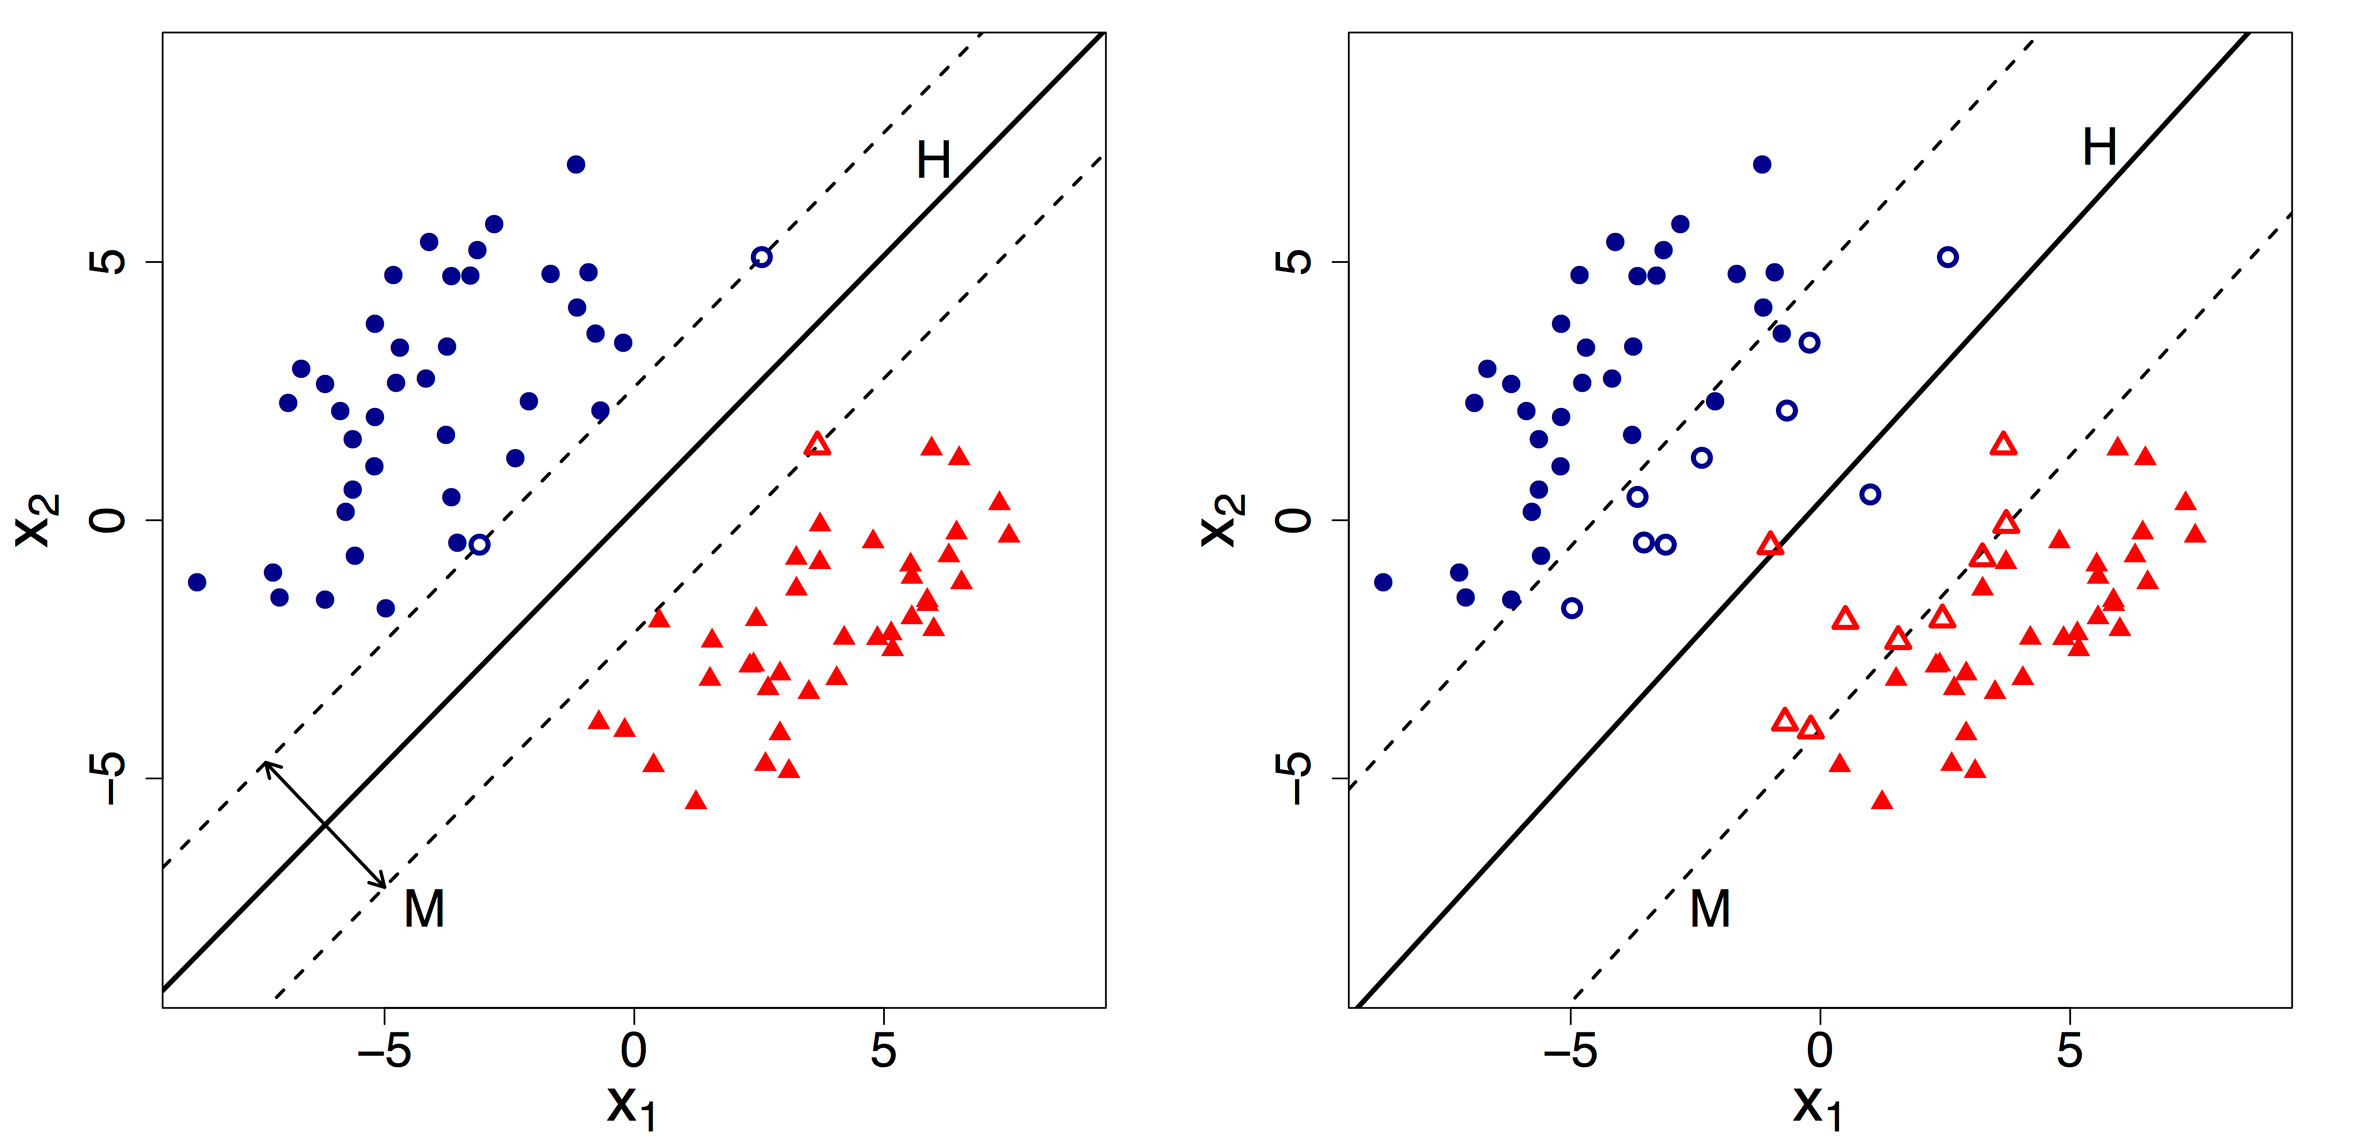
\includegraphics[width=0.7\linewidth]{pictures/svm}
		\caption{SVM decision boundary with 2 classes.
		\emph{Left}: Linearly separable, no rule violations ($C=0$).
		\emph{Right}: Not perfectly linearly separable, soft margins ($C>0$)}
		\label{fig:svm_decision_boundary}
	\end{figure}

	\paragraph{Details of the support vector classifier (SVC)}
	The support vector classifier is the solution to the following optimization problem.
	\begin{equation}
	\begin{split}
		&\text{maximize M}\\
		&\text{subject to}\sum_{j=1}^{p}\beta_{j}^2=1\\
		&y_{i}(\beta_{0}+\beta_{1}x_{i1}+\beta_{2}x_{i2}+...+\beta_{p}x_{ip})\ge M(1-\epsilon_{i})\\
		&\epsilon_{i}\ge 0, \sum_{i=1}^{n}\epsilon_{i}\ge C
	\end{split}
	\end{equation}
	\textbf{C} is the budget how many "rule violations" and how much uncertainty is allowed in total. The optimal C is found with cross validation.

	\textbf{Support vectors} are all datapoints which fall on the lines of the decision margin.

	$\epsilon$ are \textbf{slack variables}. Each training observation has a slack variable associated which allows this observation to violate the margin or even be on the wrong side of the hyperplane.
	\begin{itemize}
		\item if $\epsilon=0$, the observation is on the correct side of the margin M
		\item if $\epsilon>0$, it is on the wrong side of the margin (uncertain)
		\item if $\epsilon<1$, it is still on the correct side of the hyperplane
		\item if $\epsilon>1$, it is on the wrong side of the hyperplane (misclassified)
	\end{itemize}

	\subsection{Support vector machines}

	\paragraph{Classification with non-linear (quadratic) decision boundaries}
	When the datapoints aren't linearly separable, a non-linear approach is used. In the past we have extended linear approaches by using higher order terms as additional predictors. So instead of using the original $p$ predictors we could also use $2p$ predictors with the power of two of the original predictors.
	\begin{equation}
	\begin{split}
		&\text{maximize M}\\
		&\text{subject to } y_{i}(\beta_{0}+\sum_{j=1}^{p}\beta_{j1}x_{ij}+\sum_{j=1}^{p}\beta_{j2}x_{ij}^2)\ge M(1-\epsilon_{i})\\
		&\sum_{i=1}^{n}\epsilon_{i}\le C, \epsilon_{i}\ge 0, \sum_{j=1}^{p}\sum_{k=1}^{2}\beta_{jk}^2=1
	\end{split}
	\end{equation}
	This will result in a linear decision boundary in the new feature space, which is a non-linear decision boundary in the original feature space. This trick can be applied endlessly however ($X^3, X^4, ...$), so a smart selection of features is required to avoid an explosion in computation.

	\paragraph{Support vector machine (SVM)}
	The SVM is an extension of the support vector classifier that results from enlarging the feature space using kernels. Kernels are a computationally efficient approach for enlarging the feature space. So far the algorithm of how the optimization problem is solved has not been discussed. As it turns out, the solution does not need the observations directly but only inner products between all pairs of training observations $\left(\begin{matrix}n\\2\end{matrix}\right)$, resulting in $n(n-1)/2$ pairs.
	\begin{equation}
	\begin{split}
		\langle x_{i},x_{i'}\rangle&=\sum_{j=1}^{p}x_{ij}x_{i'j}\\
		f(x)=\beta_{0}&+\sum_{i=1}^{n}\alpha_{i} \langle x,x_{i}\rangle\\
		\alpha_i: \text{ weight of }&x_i\text{ as a support vector}\\
	\end{split}
	\end{equation}
	$\alpha_{i}$ is only non-zero for the support vectors, hence the formula can be simplified by defining $S$:
	\begin{equation}
	\begin{split}
		S: \text{ support vector indices}\\
		f(x)=\beta_{0}+\sum_{i\in S}\alpha_{i}\langle x,x_{i}\rangle
	\end{split}
	\end{equation}
	Both $f(x)$ and $\alpha_i$ only require inner products. Hence if the extension to a non-linear decision boundary generalizes the inner product calculation, then the original algorithm for solving the linear support vector classifier optimization problem can still be used. This is called the \textbf{kernel trick}. The generalization of the inner product using a so called \textbf{kernel}.
	\begin{equation}
	\begin{split}
		&K(x_{i},x_{i'})=\sum_{j=1}^{p}x_{ij}x_{i'j} \qquad \textbf{linear kernel}\\
		&K(x_{i},x_{i'})=\left(1+\sum_{j=1}^{p}x_{ij}x_{i'j}\right)^d \qquad \textbf{kernel of degree }d
	\end{split}
	\end{equation}
	If $d>1$ is used in finding $\alpha$ and in the evaluation of the classifier function, then the support vector classifier gains in flexibility via a non-linear decision boundary, making it a \textbf{Support vector machine} with the following function:
	\begin{equation}
		f(x)=\beta_{0}+\sum_{i\in S}\alpha_{i}K(x,x_{i})
	\end{equation}

	\paragraph{The advantage of the kernel trick} over explicitly enlarging the feature space is computation, since $\alpha$ can be calculated using only the kernel function and does not need to operate in the enlarged feature space.

	\subsection{SVMs with more than 2 classes}
	So far all scheme discussed in this chapter were binary classification schemes. We need an extension to the basic approach. Unfortunately, the concept of a separating hyperplane has no natural extension to the case of more than two classes. There are several extensions to the K-class problem and all of them break the K-class problem into a series of binary problems, for which an SVM is well suited. The most popular approaches are one-versus-one and one-versus-all.

	\paragraph{One-versus-one}
	The one-versus-one approach to the K-class classification problem constructs K choose 2 binary SVMs. Hence we build (K-1)K/2 SVMs. Each SVM compares a pair of classes and so each SVM is trained for that pair of classes. After all SVMs have been trained, each SVM runs to select one of the two possible classes. Of all results, the class that is picked most often is assigned to the test observation. This scheme has a problem, when more than one class has the same maximum number of calls. Every SVM can have another kernel.

	\paragraph{One-versus-all}
	The one-versus-all creates K binary SVMs, where for each SVM one of the K classes is class +1 and all the other training samples are class -1. Now instead of simply focusing on the sign of the decision function for each class, now the function value becomes important too. The class, which results in the larges decision function is assigned to the test observation. Every SVM needs the same kernel, so that it can be compared.

	\subsection{Relationship to logistic regression}
	The original optimization problem for the support vector classifier can be rewritten:
	\begin{equation}
		\text{minimize}(\sum_{i=1}^{n}max(0,1-y_{i}f(x_{i}))+\lambda\sum_{j=1}^{p}\beta_{j}^2)
	\end{equation}
	When $\lambda$ is large then $\beta_{1},...,\beta_{p}$ are small, more violation to the margin are tolerated and a low variance but high bias classifier results. Hence a small value of $\lambda$ leads to a small value of C. Since the loss functions are quite similar support vector classifier and logistic regression often give similar results. When the classes are well separated, then the support vector classifier tends to perform better, while when the classes overlap, logistic regression tends to perform better.
\end{document}
